\section{PID-Regler}

\begin{outline}
    \1 \textbf{P}: Proportional $K_p \cdot e(t)$
        \2 Gegenwart: Gewichtung des \textbf{aktuellen} Fehlers $e(t)$
            \3 Stellgrösse $u(t)$ ist abhängig vom aktuell vorhandenen Fehler
            \3 Wie gross Fehler in Vergangenheit war oder in welche Richtung er sich entwickelt, ist irrelevant
    \1 \textbf{I}: Integral $K_I \int e(t)$
        \2 Vergangenheit: Gewichtung der \textbf{Summe vergangener} Fehler
            \3  Stellgrösse $u(t)$ ist abhängig davon, wie lange ein Fehler schon existiert
            \3 Wie gross der aktuelle Fehler ist und wie start er sich gerade ändert, ist irrelevant
    \1 \textbf{D}: Differential $K_D \cdot \dot{e}(t)$
        \2 Zukunft, Trend: Gewichtung der \textbf{Änderung} des Fehlers
            \3 Stellgrösse ist abhängig davon, wie stark der Fehler gerade zu-/abnimmt
            \3 Wie gros der aktuelle Fehler ist und wie lange er schon existiert, ist irrelevant
\end{outline}


\subsection{Aufbau und Struktur}

\begin{minipage}{0.48\columnwidth}
    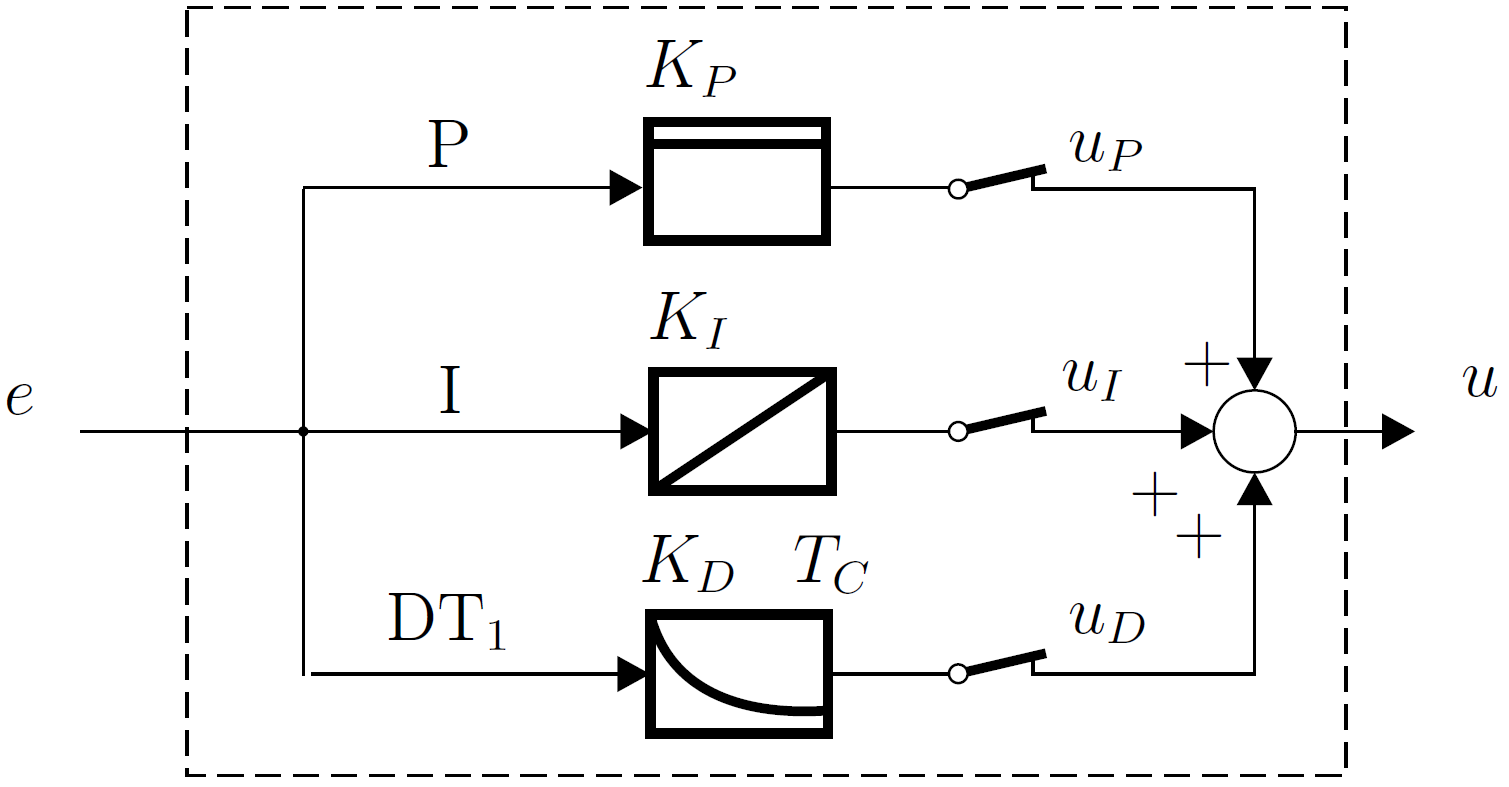
\includegraphics[width=\columnwidth]{images/pid_regler_aufbau.png}
\end{minipage}
\hfill
\begin{minipage}{0.48\columnwidth}
    \begin{center}
        \textbf{Frequenzgang realer PID-Regler}
    \end{center}
    $$ \boxed{ G_{PID}(\jimg \omega) = K_P + \frac{K_I}{\jimg \omega} + K_D \frac{\jimg \omega}{1 + \jimg \omega T_C} } $$
\end{minipage}